\graphicspath{{chapters/introduction/figures/}}


\subsection{Motivations}

\begin{frame}{Motivations}
  % \frametitle{Introduction}
  % \framesubtitle{Motivations}
  \begin{block}{\small Statistics}
    \begin{figure}%
      \centering
      \hspace*{\fill}%
      \subfigure[][\tiny \# of cancer cases]{%
        \label{fig:stat1a}%
          \includegraphics[width=.45\textwidth]{./images/statistics/repartitionCancerIncidence.png}}%
      \hfill%
      \subfigure[][\tiny \# of cancer deaths]{%
        \label{fig:stat1b}%
          \includegraphics[width=.45\textwidth]{./images/statistics/repartitionCancerDeaths.png}}%
        \hspace*{\fill}%
      \label{fig:stat1}%
    \end{figure}
  \end{block}
  \begin{block}{\small Implications}\footnotesize
    \begin{itemize}
      \item 1.4 million cases per year
      \item 10.9\% of diagnosed cancers
      \item 5\textsuperscript{th} cause of cancer death (1\textsuperscript{th} females)
    \end{itemize}
  \end{block}
\end{frame}

\subsection{Screening}

\begin{frame}{Breast Imaging}
  % \frametitle{Introduction}
  % \framesubtitle{Screening}
  \begin{block}{\small Ultra-Sound(US) imaging, the most common adjunct modality}\footnotesize
    \begin{itemize}
    \item Ability to discern solid lesions typologies
    \item Lesions shielded by dense breast in Digital Mammography(DM) are distinguishable in US
    \end{itemize}
  \end{block}

  \begin{figure}%
     \centering
     \hspace*{\fill}%
     \subfigure[][\tiny DM]{%
       \label{fig:shielda}%
     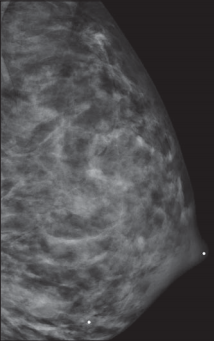
\includegraphics[trim = 0 0 0 20, clip,height=3.3cm]{mamo-us1.png}}
     \hfill%
     \subfigure[][\tiny DM, Region of Interest (ROI) ]{%
       \label{fig:shieldb}%
     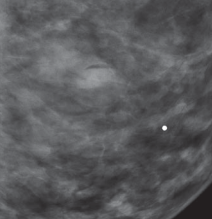
\includegraphics[trim = 0 0 0 20, clip,height=3.3cm]{mamo-us2.png}}
     \hfill%
     \subfigure[][\tiny Breast Ultra-Sound(BUS), ROI]{%
       \label{fig:shieldc}%
     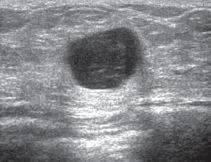
\includegraphics[trim = 10 20 10 0, clip,height=3.3cm]{mamo-us3.png}}
       \hspace*{\fill}%
    \label{fig:shield}%
  \end{figure}

\end{frame}

\subsection{Image formation, limitations and imaging perspectives}
\begin{frame}\frametitle{Breast structures under US screening}
\begin{columns}
\begin{column}{.48\textwidth}\vspace{-17pt}%\hspace{-1cm}
\begin{figure}\centering
\begin{tikzpicture}[scale=.5]
\begin{scriptsize}
	\tikzset{dot/.style={circle,draw=black,inner sep=0mm,minimum size=4pt}}
    \node[anchor=south west,inner sep=0] at (.2,.2) {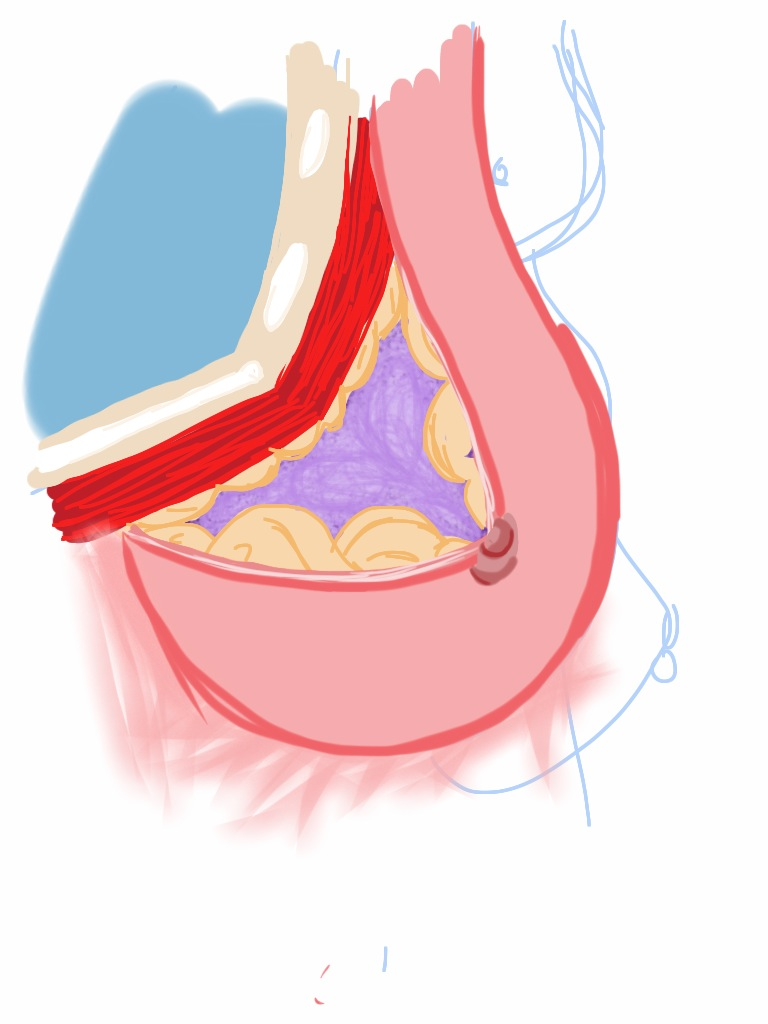
\includegraphics[trim = 20 190 80 20, clip,height=\textwidth]{pit.jpg}};
    \draw		(1.75,	7.75	) 	node[dot]	(AirCoord)			{}	
    				(2.5	,	5		) 	node[dot]	(PecCoord)			{}
    				(3.75,  7.75	) 	node[dot]	(CWCoord)			{}
    				(5,		5.40	) 	node[dot]	(TissueCoord)	{}
    				(2.5	,	3.65	) 	node[dot]	(SkinCoord)		{}
    				(3.75, 3.8	)  	node[dot]	(CooperCoord)	{}
    				(5.80, 5.40	)  	node[dot]	(FatCoord)			{};
 	   				
\draw	(AirCoord)	node[above left] (AirName) {Lungs (air)}
			node[below =of AirName.west, anchor=west] (PecName){Pectoral muscle}
   			(4.5,9.5)	node[anchor=west] (CWName){Chest-wall}
			node[below = of CWName,anchor=west,text width=2cm] (TissueName){Fibro-glandular tissue}
%    			(SkinCoord)
    			node[below= 1.8 of PecName.west, anchor=west ] (SkinName){Skin layers}
    			(CooperCoord |- SkinName)	node[text width=1.5cm,anchor= north west,inner sep=0mm,xshift=-5pt] (CooperName){Cooper's ligament}
    			(FatCoord) node[xshift=9,inner sep=0mm,anchor=west,text width=2cm] (FatName){Adipose tissue \emph{fat lobe}}
;   					 	
    \draw 	(PecCoord) -- (PecName)
    		   	(SkinCoord) -- (SkinName) 
				(CooperCoord) -- (CooperName)
%				(AirCoord) -- (AirName.south)
				(CWCoord) -- (CWName)
				(TissueCoord) -- (TissueName.west)
				(FatCoord) -- (FatName)
				;
%    
%    \draw[help lines,xstep=.5,ystep=.5] (0,0) grid (10,10);
%\foreach \x in {0,1,...,10} { \node [anchor=north] at (\x,0) {\x}; }
%\foreach \y in {0,1,...,10} { \node [anchor=east] at (0,\y) {\y}; });
\end{scriptsize}
\end{tikzpicture}
		\caption{Breast structure elements.}
		\end{figure}	
\end{column}

\begin{column}{.48\textwidth}
\begin{figure}
		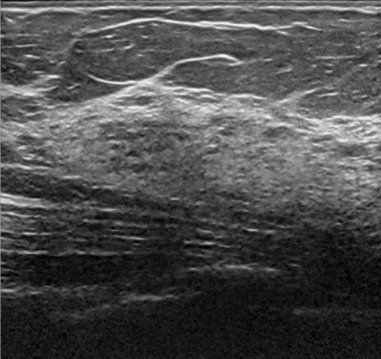
\includegraphics[height=.515\textheight]{sa1.png}
\caption{ Breast US image example.}
		\end{figure}	
\end{column}
\end{columns}
\end{frame}

\subsection{Image inspection to infer state of health}
%\subsection{Computer Aided Diagnosis (CAD)}

\begin{frame}\frametitle{State of health from image visual Inspection}
\setbeamercovered{transparent}
\begin{block}{Radiologic diagnosis error rates are similar to any other human visual inspection}
  \begin{itemize}
    \item Quality of the images.
    \item Ability to interpret the physical properties of the images.
  \end{itemize}
\end{block}
  \begin{enumerate}
    \item Double readings.
    \item Computer Aided Diagnosis(CAD).
  \end{enumerate}
\end{frame}


\definecolor{colorTheme}{RGB}{51,41,178}
\begin{frame}\frametitle{BI-RADs Lexicon}
  \framesubtitle{A standardized toolkit tested for diagnosis}
  \footnotesize
\begin{itemize}
\vspace{-5pt}
\item BKGD Echotexture :
			adipose, fibro-glandular, heterogeneous
\item Mass shape :
	\begin{tikzpicture}[baseline=(label.north)]
	\coordinate (rect) at (.5,.5);
	\coordinate (aux) at (.5,.53);

	\begin{tiny}
		\draw (0,0) rectangle (rect);
		\draw (0.25,0) node[minimum width=1cm,anchor=north](label){Oval};
		\draw [thick,colorTheme!80!white] (0.25,0.25) ellipse ( .2 and .08);
	\end{tiny}
	
	\begin{pgfonlayer}{background}
	\fill [green!30,rounded corners=2pt] ($ (label.west) !.65! (label.south west) $) rectangle (aux -| label.east);
	\end{pgfonlayer}
	\end{tikzpicture}
		\begin{tikzpicture}[baseline=(label.north)]
	\coordinate (rect) at (.5,.5);
	\coordinate (aux) at (.5,.53);

	\begin{tiny}
		\draw (0,0) rectangle (rect);
		\draw (0.25,0) node[minimum width=1cm,anchor=north](label){Round};
%				   (.25,.25) circle[fill,radius=.18,fill=red];
		\draw [thick,colorTheme!80!white]   (.25,.25) circle[radius=.18];
	\end{tiny}
	
	\begin{pgfonlayer}{background}
	\fill [red!30,rounded corners=2pt] ($ (label.west) !.65! (label.south west) $) rectangle (aux -| label.east);
	\end{pgfonlayer}
	\end{tikzpicture} 
		\begin{tikzpicture}[baseline=(label.north)]
	\coordinate (rect) at (.5,.5);
	\coordinate (aux) at (.5,.53);

	\begin{tiny}
		\draw (0,0) rectangle (rect);
		\draw (0.25,0) node[minimum width=1cm,anchor=north](label){Irregular};
		\draw [thick,colorTheme!80!white,rounded corners=2pt]   (.05,.25) -- (.1, .1)  -- (.2,.3) -- (.3,.2)  -- (.2,.05) -- (.35,.06) -- (.45,.25) -- (.4,.46) -- (.15,.3) -- (.1,.45) -- cycle;		
	\end{tiny}
	
	\begin{pgfonlayer}{background}
	\fill [red!30,rounded corners=2pt] ($ (label.west) !.65! (label.south west) $) rectangle (aux -| label.east);
	\end{pgfonlayer}
	\end{tikzpicture}
		\begin{tikzpicture}[baseline=(label.north)]
	\coordinate (rect) at (.5,.5);
	\coordinate (aux) at (.5,.53);

	\begin{tiny}
		\draw (0,0) rectangle (rect);
		\draw (0.25,0) node[minimum width=1cm,anchor=north](label){Lobular};
		\draw [thick,colorTheme!80!white,rounded corners=2pt]   (.05,.25) -- (.18,.15) -- (.25,.25) -- (.35,.15) -- (.45,.25) -- (.35,.35) -- (.25,.25) -- (.18,.35) -- cycle;
	\end{tiny}
	
	\begin{pgfonlayer}{background}
	\fill [orange!30,rounded corners=2pt] ($ (label.west) !.65! (label.south west) $) rectangle (aux -| label.east);
	\end{pgfonlayer}
	\end{tikzpicture}
\item Mass orientation :
		\begin{tikzpicture}[baseline=(label.north)]
	\coordinate (rect) at (.5,.5);
	\coordinate (aux) at (.5,.53);

	\begin{tiny}
		\draw (0,0) rectangle (rect);
		\draw (0.25,0) node[minimum width=1cm,anchor=north](label){Parallel};
		\draw[gray] (0,.44) -- (.5,.44);
		\draw[gray] (0,.47) -- (.5,.47);
		\draw [thick,colorTheme!80!white] (0.25,0.25) ellipse ( .15 and .06);
	\end{tiny}
	
	\begin{pgfonlayer}{background}
	\fill [green!30,rounded corners=2pt] ($ (label.west) !.65! (label.south west) $) rectangle (aux -| label.east);
	\end{pgfonlayer}
	\end{tikzpicture}
		\begin{tikzpicture}[baseline=(label.north)]
	\coordinate (rect) at (.5,.5);
	\coordinate (aux) at (.5,.53);

	\begin{tiny}
		\draw (0,0) rectangle (rect);
		\draw (0.25,0) node[anchor=north](label){Non-parallel};
		\draw[gray] (0,.44) -- (.5,.44);
		\draw[gray] (0,.47) -- (.5,.47);
		\draw [thick,colorTheme!80!white] (0.25,0.25) ellipse ( .06 and .15);
	\end{tiny}
	
	\begin{pgfonlayer}{background}
	\fill [red!30,rounded corners=2pt] ($ (label.west) !.65! (label.south west) $) rectangle (aux -| label.east);
	\end{pgfonlayer}
	\end{tikzpicture}
\item Mass margin :
		\begin{tikzpicture}[baseline=(label.north)]
	\coordinate (rect) at (.5,.5);
	\coordinate (aux) at (.5,.53);

	\begin{tiny}
		%\draw (0,0) rectangle (rect);
		\node[inner sep=0pt,anchor=south west]  at (0,0) {
\includegraphics[height=.5cm]{birads/circumscribed}};
		\draw (0.25,0) node[minimum width=1cm,anchor=north](label){Circumscribed};
	\end{tiny}
	
	\begin{pgfonlayer}{background}
	\fill [green!30,rounded corners=2pt] ($ (label.west) !.65! (label.south west) $) rectangle (aux -| label.east);
	\end{pgfonlayer}
	\end{tikzpicture}
		\begin{tikzpicture}[baseline=(label.north)]
	\coordinate (rect) at (.5,.5);
	\coordinate (aux) at (.5,.53);

	\begin{tiny}
		\node[inner sep=0pt,anchor=south west]  at (0,0) {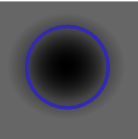
\includegraphics[height=.5cm]{birads/indistinct.png}};
		\draw (0.25,0) node[minimum width=1cm,anchor=north](label){Indistinct};
	\end{tiny}
	
	\begin{pgfonlayer}{background}
	\fill [red!30,rounded corners=2pt] ($ (label.west) !.65! (label.south west) $) rectangle (aux -| label.east);
	\end{pgfonlayer}
	\end{tikzpicture}
		\begin{tikzpicture}[baseline=(label.north)]
	\coordinate (rect) at (.5,.5);
	\coordinate (aux) at (.5,.53);

	\begin{tiny}
		\draw (0,0) rectangle (rect);
		\node[inner sep=0pt,anchor=south west]  at (.03,.12) {
\includegraphics[height=.3cm]{birads/angular}};
		\draw (0.25,0) node[minimum width=1cm,anchor=north](label){Angular};
	\end{tiny}
	
	\begin{pgfonlayer}{background}
	\fill [red!30,rounded corners=2pt] ($ (label.west) !.65! (label.south west) $) rectangle (aux -| label.east);
	\end{pgfonlayer}
	\end{tikzpicture}
		\begin{tikzpicture}[baseline=(label.north)]
	\coordinate (rect) at (.5,.5);
	\coordinate (aux) at (.5,.53);

	\begin{tiny}
			\draw (0,0) rectangle (rect);
		\node[inner sep=0pt,anchor=south west]  at (.05,.12) {
\includegraphics[height=.3cm]{birads/micro.pdf}};
		\draw (0.25,0) node[minimum width=1cm,anchor=north](label){Microlobulated};
	\end{tiny}
	
	\begin{pgfonlayer}{background}
	\fill [red!30,rounded corners=2pt] ($ (label.west) !.65! (label.south west) $) rectangle (aux -| label.east);
	\end{pgfonlayer}
	\end{tikzpicture}
		\begin{tikzpicture}[baseline=(label.north)]
	\coordinate (rect) at (.5,.5);
	\coordinate (aux) at (.5,.53);

	\begin{tiny}
		\draw (0,0) rectangle (rect);
		\node[inner sep=0pt,anchor=south west]  at (0.06,0.1) {
\includegraphics[height=.35cm]{birads/spiculated}};
		\draw (0.25,0) node[minimum width=1cm,anchor=north](label){Spiculated};
	\end{tiny}
	
	\begin{pgfonlayer}{background}
	\fill [red!30,rounded corners=2pt] ($ (label.west) !.65! (label.south west) $) rectangle (aux -| label.east);
	\end{pgfonlayer}
	\end{tikzpicture}
\item Lesion boundary :
		\begin{tikzpicture}[baseline=(label.north)]
	\coordinate (rect) at (.5,.5);
	\coordinate (aux) at (.5,.53);

	\begin{tiny}
%		\draw (0,0) rectangle (rect);
		\node[inner sep=0pt,anchor=south west]  at (0,0) {
\includegraphics[height=.5cm]{birads/Abrupt}};
		\draw (0.25,0) node[minimum width=1cm,anchor=north](label){Abrupt Interface};
	\end{tiny}
	
	\begin{pgfonlayer}{background}
	\fill [green!30,rounded corners=2pt] ($ (label.west) !.65! (label.south west) $) rectangle (aux -| label.east);
	\end{pgfonlayer}
	\end{tikzpicture}
		\begin{tikzpicture}[baseline=(label.north)]
	\coordinate (rect) at (.5,.5);
	\coordinate (aux) at (.5,.53);

	\begin{tiny}
%		\draw (0,0) rectangle (rect);
		\node[inner sep=0pt,anchor=south west]  at (0,0) {
\includegraphics[height=.5cm]{birads/halo}};
		\draw (0.25,0) node[minimum width=1cm,anchor=north](label){Echogenic halo};
	\end{tiny}
	
	\begin{pgfonlayer}{background}
	\fill [red!30,rounded corners=2pt] ($ (label.west) !.65! (label.south west) $) rectangle (aux -| label.east);
	\end{pgfonlayer}
	\end{tikzpicture}
\item Echo pattern :
		\begin{tikzpicture}[baseline=(label.north)]
	\coordinate (rect) at (.5,.5);
	\coordinate (aux) at (.5,.53);

	\begin{tiny}
		\node[inner sep=0pt,anchor=south west]  at (0,0) {
\includegraphics[height=.5cm]{birads/anechoic}};
		\draw (0.25,0) node[minimum width=1cm,anchor=north](label){Anechoic};
	\end{tiny}
	
	\begin{pgfonlayer}{background}
	\fill [green!30,rounded corners=2pt] ($ (label.west) !.65! (label.south west) $) rectangle (aux -| label.east);
	\end{pgfonlayer}
	\end{tikzpicture}
		\begin{tikzpicture}[baseline=(label.north)]
	\coordinate (rect) at (.5,.5);
	\coordinate (aux) at (.5,.53);

	\begin{tiny}
		\node[inner sep=0pt,anchor=south west]  at (0,0) {
\includegraphics[height=.5cm]{birads/hyperechoic}};
		\draw (0.25,0) node[minimum width=1cm,anchor=north](label){Hyperechoic};
	\end{tiny}
	
	\begin{pgfonlayer}{background}
	\fill [green!30,rounded corners=2pt] ($ (label.west) !.65! (label.south west) $) rectangle (aux -| label.east);
	\end{pgfonlayer}
	\end{tikzpicture}
		\begin{tikzpicture}[baseline=(label.north)]
	\coordinate (rect) at (.5,.5);
	\coordinate (aux) at (.5,.53);

	\begin{tiny}
\node[inner sep=0pt,anchor=south west]  at (0,0) {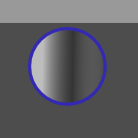
\includegraphics[height=.5cm]{birads/complex.png}};
		\draw (0.25,0) node[minimum width=1cm,anchor=north](label){Complex};
	\end{tiny}
	
	\begin{pgfonlayer}{background}
	\fill [red!30,rounded corners=2pt] ($ (label.west) !.65! (label.south west) $) rectangle (aux -| label.east);
	\end{pgfonlayer}
	\end{tikzpicture}
		\begin{tikzpicture}[baseline=(label.north)]
	\coordinate (rect) at (.5,.5);
	\coordinate (aux) at (.5,.53);

	\begin{tiny}
%		\draw (0,0) rectangle (rect);
		\node[inner sep=0pt,anchor=south west]  at (0,0) {
\includegraphics[height=.5cm]{birads/isoechoic}};
		\draw (0.25,0) node[minimum width=1cm,anchor=north](label){Isoechoic};
	\end{tiny}
	
	\begin{pgfonlayer}{background}
	\fill [orange!30,rounded corners=2pt] ($ (label.west) !.65! (label.south west) $) rectangle (aux -| label.east);
	\end{pgfonlayer}
	\end{tikzpicture}
		\begin{tikzpicture}[baseline=(label.north)]
	\coordinate (rect) at (.5,.5);
	\coordinate (aux) at (.5,.53);

	\begin{tiny}
		\node[inner sep=0pt,anchor=south west]  at (0,0) {
\includegraphics[height=.5cm]{birads/hypoechoic}};
		\draw (0.25,0) node[minimum width=1cm,anchor=north](label){Hypoechoic};
	\end{tiny}
	
	\begin{pgfonlayer}{background}
	\fill [orange!30,rounded corners=2pt] ($ (label.west) !.65! (label.south west) $) rectangle (aux -| label.east);
	\end{pgfonlayer}
	\end{tikzpicture}
\item Posterior acoustic pattern : 
		\begin{tikzpicture}[baseline=(label.north)]
	\coordinate (rect) at (.5,.5);
	\coordinate (aux) at (.5,.53);

	\begin{tiny}
\node[inner sep=0pt,anchor=south west]  at (0,0) {
\includegraphics[height=.5cm]{birads/shadow}};
		\draw (0.25,0) node[minimum width=1cm,anchor=north](label){Shadowing};
	\end{tiny}
	
	\begin{pgfonlayer}{background}
	\fill [red!30,rounded corners=2pt] ($ (label.west) !.65! (label.south west) $) rectangle (aux -| label.east);
	\end{pgfonlayer}
	\end{tikzpicture}
		\begin{tikzpicture}[baseline=(label.north)]
	\coordinate (rect) at (.5,.5);
	\coordinate (aux) at (.5,.53);

	\begin{tiny}
\node[inner sep=0pt,anchor=south west]  at (0,0) {
\includegraphics[height=.5cm]{birads/combined}};
		\draw (0.25,0) node[minimum width=1cm,anchor=north](label){Combined};
	\end{tiny}
	
	\begin{pgfonlayer}{background}
	\fill [red!30,rounded corners=2pt] ($ (label.west) !.65! (label.south west) $) rectangle (aux -| label.east);
	\end{pgfonlayer}
	\end{tikzpicture}
		\begin{tikzpicture}[baseline=(label.north)]
	\coordinate (rect) at (.5,.5);
	\coordinate (aux) at (.5,.53);

	\begin{tiny}
\node[inner sep=0pt,anchor=south west]  at (0,0) {
\includegraphics[height=.5cm]{birads/enhance}};
		\draw (0.25,0) node[minimum width=1cm,anchor=north](label){Enhancement};
	\end{tiny}
	
	\begin{pgfonlayer}{background}
	\fill [orange!30,rounded corners=2pt] ($ (label.west) !.65! (label.south west) $) rectangle (aux -| label.east);
	\end{pgfonlayer}
	\end{tikzpicture}
		\begin{tikzpicture}[baseline=(label.north)]
	\coordinate (rect) at (.5,.5);
	\coordinate (aux) at (.5,.53);

	\begin{tiny}
\node[inner sep=0pt,anchor=south west]  at (0,0) {
\includegraphics[height=.5cm]{birads/hypoechoic}};
		\draw (0.25,0) node[minimum width=1cm,anchor=north](label){No pattern};
	\end{tiny}
	
	\begin{pgfonlayer}{background}
	\fill [orange!30,rounded corners=2pt] ($ (label.west) !.65! (label.south west) $) rectangle (aux -| label.east);
	\end{pgfonlayer}
	\end{tikzpicture}
\end{itemize}

\footnotetext{~\tikz[baseline=(x),inner sep=1.5pt] {\coordinate (x) at (0,-3pt); \node[fill=green!30,rounded corners=2pt,anchor=base,minimum size=10pt] {};} benign, \tikz[baseline=(x),inner sep=1.5pt] {\coordinate (x) at (0,-3pt); \node[fill=red!30,rounded corners=2pt,anchor=base,minimum size=10pt] {};} malignant and \tikz[baseline=(x),inner sep=1.5pt] {\coordinate (x) at (0,-3pt); \node[fill=orange!30,rounded corners=2pt,anchor=base,minimum size=10pt] {};} undetermined 
  \\
\vspace{2pt}}
\end{frame}

\begin{frame}\frametitle{Take away}
  \framesubtitle{Accurate delineations to develop CAD systems for BUS}
\begin{figure}
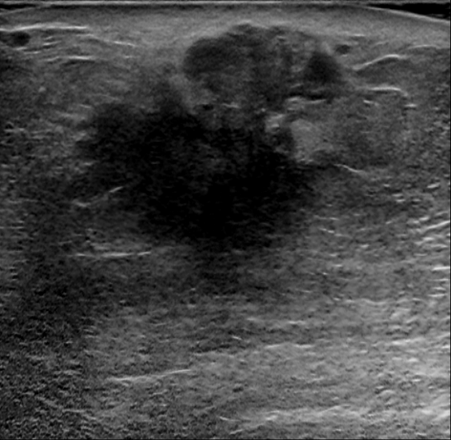
\includegraphics[trim=0 6 0 0,clip,height=.5\textheight]{a110105_094.png}~
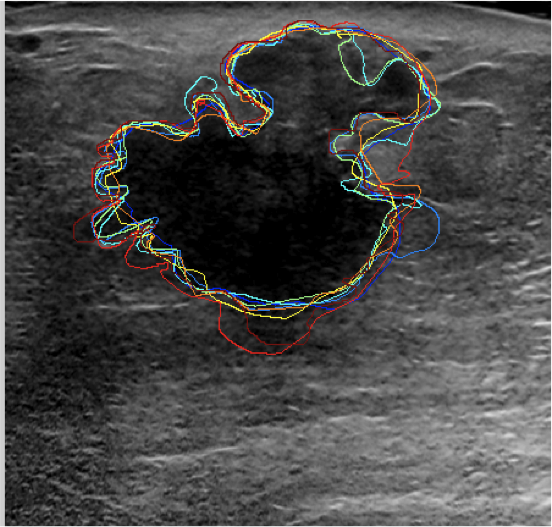
\includegraphics[trim=6 0 0 0,clip,height=.5\textheight]{segment.png}
\end{figure}
\end{frame}
